\documentclass[12pt]{article}

% Load necessary packages
\usepackage{geometry}
\usepackage{graphicx}
\usepackage{hyperref}
\usepackage{listings}
\usepackage{xcolor}
\usepackage[utf8]{inputenc}
\usepackage{hyperref}

% Set page margins
\geometry{left=3cm, right=3cm, top=2cm, bottom=2cm}

% Define colors for hyperlinks
\hypersetup{
    colorlinks=true,
    linkcolor=black,
    filecolor=black,
    urlcolor=black,
    citecolor=black
}

\begin{document}

\begin{titlepage}
    \centering
    % \includegraphics[width=0.8\textwidth]{image.jpeg}\par
    % % \includegraphics[width=14cm]{image.png} % Replace 'path_to_your_image.jpg' with the actual file path
    \begin{figure}[h] % You can specify the placement options (h = here, t = top, b = bottom, etc.)
    \centering      % Center the contents of the figure environment
    \includegraphics[width=0.9\textwidth]{logo.png}
    \label{fig2}
    \end{figure}
    \vspace{2cm}
    {\scshape\Large SOEN6841: Topic Analysis and Synthesis Report \par}
    \vspace{1.5cm}
    {\scshape\Huge How to Share Decisions for Strong Execution\par}
    \vspace{1.5cm}
    % {\large Advisor: Professor Pankaj Kamthan\par}
    \vspace{0.5cm}
    {\large By: Brinda Pareshbhai Patel (Student ID: 40218974)\par}
    \vspace{2.5cm}
    \textbf{\large Under the Guidance of}\\[0.15in]
    Prof. Pankaj Kamthan\\[0.4in]
    \vspace{1cm}
    {\large \today\par}
\end{titlepage}

% Table of Contents
\tableofcontents
\newpage

% Abstract Section
\section*{Abstract}

Effective decision-making and communication within teams are fundamental to strong execution and team alignment. This paper, drawing insights from Katie Womersley's case study, delves into various strategies for enhancing decision-sharing processes in organizational settings. Central to these strategies is the necessity of clarifying decisions, a step that mitigates the risk of misinterpretation and ensures a unified understanding across the team. This involves articulating decisions in a clear, unambiguous manner and avoiding assumptions about common knowledge.\\
\\The study further emphasizes the importance of preemptive communication about decision-making processes. By informing team members about upcoming decisions, the study argues for a more inclusive environment where diverse viewpoints can be considered, particularly benefiting those who require time for contemplation. This approach aids in preparing the team and in gathering a wider range of perspectives, thereby enriching the decision-making process.\\
\\Additionally, the study highlights the role of clear designation of decision-makers. Using tools such as the RACI matrix, it underscores the need to identify and communicate who is responsible for making decisions. This clarity not only fosters accountability but also prevents the bystander effect, ensuring that decisions are not only made but also owned by specific individuals or groups within the team.\\
\\The necessity of documenting decisions is also discussed. The study advocates for recording decisions in an accessible and persistent format, such as a digital document, facilitating future references and ensuring consistency in understanding and implementation. This documentation process serves as a reference point for all team members, aiding in aligning actions with decisions.\\
\\Finally, the study addresses the challenge of time investment in communication. It argues that while thorough and proactive communication can be time-consuming, it is far less costly than the repercussions of miscommunication, such as redoing work or mending strained relationships. It concludes that a team aligned in understanding and direction through effective communication and decision-sharing is more efficient and effective in achieving its objectives.\\

\newpage

\section{Introduction}

\subsection{Problem Statement}
The research questions guiding this investigation are:
\begin{itemize}
  \item How can leaders ensure decisions are understood clearly by all team members to avoid ambiguity?
  \item What methods can be used to inform the team about significant decision-making processes?
  \item How should the roles of decision-makers be communicated within a team to ensure efficiency and accountability?
  \item What are the best practices for documenting decisions to facilitate future reference and maintain clarity?
  \item Which communication techniques are most effective in conveying decisions to a diverse team or organization?
\end{itemize}


\subsection{Motivation}
\begin{itemize}
  \item The growing prevalence of remote work environments and distributed teams in modern organizations.
  \item Challenges in decision-making processes and communication in non-collocated teams.
  \item The need for structured and transparent decision-making methods to enhance team alignment and efficiency.
  \item The importance of documentation and clear communication in decentralized team structures.
\end{itemize}


\subsection{Objectives}
\begin{itemize}
  \item To delineate best practices for decision making and communication in distributed teams.
  \item To provide insights into effective use of tools and methodologies like RACI matrices for enhancing team clarity and coordination.
  \item To guide team leaders and members in adopting strategies that support better decision-making and communication in a remote setup.
\end{itemize}

\section{Background Material}

\subsection{Subject 1: Environmental Impact Assessment in Chinese Infrastructure}
\begin{itemize}
  \item The Environmental Impact Assessment (EIA) in China's expressway infrastructure focuses on the decision-making hierarchy and its environmental implications \cite{reference1}.
  \item This area of study is crucial for understanding the structured processes of decision-making in large-scale infrastructure projects, with a particular emphasis on environmental sustainability.
\end{itemize}

\subsection{Subject 2: Shared Decision Making in Healthcare}
\begin{itemize}
  \item Coulter's research highlights the importance of shared decision-making in healthcare, discussing the challenges and benefits of collaborative processes in patient care \cite{reference2}.
  \item This study is pertinent for understanding the dynamics and effectiveness of decision-making in environments with multiple stakeholders, emphasizing the role of communication in achieving consensus.
\end{itemize}

\subsection{Subject 3: Strategic Decision-Making Processes}
\begin{itemize}
  \item Analyzing the role of management and context in strategic decision-making processes, this study provides insights into the influence of various managerial approaches and environmental factors on organizational decisions \cite{reference4}.
  \item The research is valuable for understanding how different strategies and contexts can impact decision-making processes within organizations.
\end{itemize}

\subsection{Subject 4: Goal Setting in Teams}
\begin{itemize}
  \item Focusing on goal clarity and team performance, this research emphasizes the importance of setting clear and defined goals for team effectiveness, especially in public sector teams \cite{reference5}.
  \item The study contributes to a deeper understanding of how well-articulated goals can enhance the performance and efficiency of teams.
\end{itemize}

\newpage

\section{Methods \& Methodology}

\subsection{Literature Review and Comparative Analysis}
\begin{itemize}
  \item Conducted a thorough review of existing literature on decision-making processes across various fields including environmental impact \cite{reference1}, healthcare \cite{reference2}, strategic business management \cite{reference4}, and team performance in the public sector \cite{reference5}.
  \item Performed comparative analysis to identify similarities and differences in decision-making strategies, challenges, and outcomes across these diverse contexts.
  \item This approach helped to synthesize broad insights and recognize patterns applicable to organizational decision-making and communication.
\end{itemize}

\subsection{Exploratory Qualitative Analysis}
\begin{itemize}
  \item Utilized an exploratory approach to delve into specific aspects such as preference for decision control in organizations \cite{reference6} and the use of decision documentation tools \cite{reference7}.\\
 \begin{figure}[h]
    \centering
     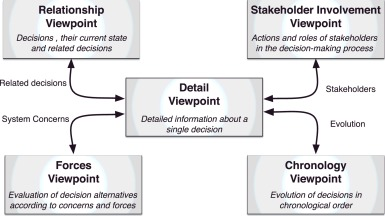
\includegraphics[width=0.7\textwidth]{viewpoints.jpg}
    \caption{The five decision viewpoints of the decision documentation framework.}
    \label{fig:figure1}
\end{figure}

  \item Conducted qualitative content analysis of case studies on team management \cite{reference8} and execution-time communication decisions \cite{reference9}, focusing on real-world applications and implications.
  \item This methodology was essential for uncovering nuanced insights and understanding the practical application of theoretical concepts.
\end{itemize}

\subsection{Framework Alignment and Theoretical Evaluation}
\begin{itemize}
  \item Aligned the findings from various studies with established decision-making frameworks and theories.
  \item Evaluated how these frameworks are adapted or challenged by the empirical evidence and case studies reviewed.
  \item This method was crucial for assessing the validity and applicability of traditional decision-making models in contemporary organizational settings.
\end{itemize}

\subsection{Data Synthesis and Thematic Analysis}
\begin{itemize}
  \item Employed thematic synthesis to draw out key themes, patterns, and insights from the accumulated data.
  \item Analyzed and coded the data to identify recurring themes related to decision-making effectiveness, communication strategies, and organizational alignment \cite{reference10}.
  \item This approach provided a structured way to distill complex information into actionable insights and recommendations.
\end{itemize}

\newpage

\section{Results Obtained}

\subsection{Under What Conditions}
\begin{itemize}
  \item The effectiveness of shared decision-making was significantly influenced by organizational culture and structure \cite{reference3}. A collaborative and open culture facilitated better decision-making.
  \item Environmental factors, such as regulatory compliance in infrastructure projects \cite{reference1}, played a crucial role in shaping decision-making processes.
  \item In healthcare, patient engagement and informed consent were critical conditions for effective shared decision-making \cite{reference2}.
\end{itemize}

\subsection{Constraints}
\begin{itemize}
  \item Time constraints often hindered thorough decision-making processes, leading to rushed or suboptimal choices \cite{reference7}.
  \item Lack of clear communication channels and decision-making authority \cite{reference6} often resulted in ambiguity and inefficiencies.
  \item Resource limitations, both in terms of manpower and technological tools, were identified as major constraints impacting decision quality \cite{reference9}.
\end{itemize}

\subsection{Quality of Decision-Making}
\begin{itemize}
  \item The overall quality of decision-making varied significantly across different organizations and contexts. In cases where strategic alignment was emphasized \cite{reference10}, decisions tended to be more effective and aligned with organizational goals.
  \item In well-structured environments with clear roles and responsibilities, as advocated by the RACI matrix, decision quality was generally adequate \cite{reference8}.
  \item However, in scenarios with poor communication and undefined decision-making processes, the quality of decisions was often subpar, leading to ineffective outcomes \cite{reference5}.
  \item The integration of comprehensive decision documentation tools \cite{reference7} contributed to improving the quality of decisions by providing a reference and accountability mechanism.
\end{itemize}

\newpage
\section{Conclusions and Future Works}

\subsection{Suggested Improvements}
In order to enhance the applicability of the solutions proposed in this study, several improvements can be considered:
\begin{itemize}
  \item Integration of advanced communication technologies: Future efforts should focus on adopting and developing advanced communication tools and platforms that facilitate real-time decision-sharing, especially in remote and distributed team settings. This could involve the use of AI-driven decision support systems.
  \item Enhanced training and education: Organizations can invest in training programs that empower team members with decision-making and communication skills. This could lead to more effective implementation of shared decision-making practices.
  \item Continuous feedback mechanisms: Establishing feedback loops for decision-making processes can enable organizations to adapt and improve over time. Regular assessments and refinements are essential for sustained success.
  \item Inclusion of decision-making in performance evaluation: Encouraging organizations to include decision-making effectiveness as a key performance metric can incentivize individuals and teams to prioritize clarity, documentation, and communication in their decision processes.
\end{itemize}

\subsection{Limitations to Solution}
While the solutions presented in this study are valuable in many organizational contexts, there are limitations to their applicability:
\begin{itemize}
  \item High-stakes, time-sensitive decisions: In situations where decisions must be made rapidly and the consequences of failure are severe, the detailed decision-making processes advocated here may not be feasible. Quick, authoritative decisions may be required.
  \item Cultural and organizational diversity: The effectiveness of shared decision-making can vary greatly across different cultures and organizations. What works well in one context may not work as effectively in another due to varying communication norms and practices.
\end{itemize}

\subsection{Applications in the Real World}
The solutions and strategies discussed in this study can be immediately applied in various real-world scenarios, including:
\begin{itemize}
  \item Healthcare institutions, where shared decision-making can lead to better patient outcomes and satisfaction.
  \item Large infrastructure projects, such as those in the construction and engineering sectors, where clear decision-making processes are crucial for project success and compliance with regulations.
  \item Public sector organizations, where goal clarity and team performance are essential for delivering effective services to the community.
\end{itemize}

\subsection{Conclusion}

\begin{enumerate}
    \item \textbf{Clarity and Communication:} The importance of clarity in decision-making cannot be overstated. It is crucial to have a clear understanding of what the decision entails to prevent misunderstandings and to ensure that all team members have a unified perspective. Equally important is the clear communication of the decision to avoid different interpretations and to ensure a cohesive team approach.

    \item \textbf{Preparation and Inclusion:} Sharing information about the decision-making process in advance allows team members to prepare appropriately. This leads to a more comprehensive and inclusive decision-making process, respecting the diverse thinking styles within a team and ensuring that decisions are well-considered and robust.

    \item \textbf{Defining Roles and Responsibilities:} Clearly identifying and communicating the roles of decision-makers, such as through a RACI matrix, helps in establishing accountability and clarity in the decision-making process. Delegating decision-making authority also empowers team members and builds a more autonomous and dynamic team.

    \item \textbf{Documentation and Accessibility:} It is essential to record decisions in a format that is both persistent and accessible, like in a shared document. This practice is vital for maintaining organizational memory and provides a reference for future decisions and actions.

    \item \textbf{Broad Sharing and Updating Relevant Materials:} Communicating decisions to all relevant stakeholders, including those indirectly affected, fosters transparency and inclusivity. Updating all relevant documents and workflows in alignment with new decisions ensures that the entire team operates with the latest information.

    \item \textbf{Efficiency vs. Expediency:} Although the decision-making process might seem time-consuming, it is significantly more efficient in the long term. Clear and comprehensive communication minimizes the risk of misalignment, confusion, and the need for rework, thus saving time and enhancing overall team productivity.
\end{enumerate}

In summary, effective decision-making and communication are not just about making the right choices but also about ensuring that these choices are clearly understood, accepted, and implemented by the entire team. This approach leads to stronger team alignment, more efficient execution of tasks, and ultimately contributes to the success of the organization.



% (Add subsequent sections like Methodology, Case Study Analysis, Conclusion, References as needed)
\begin{thebibliography}{8}
\addcontentsline{toc}{section}{References}
    \bibitem{reference1}
    EIA application in China’s expressway infrastructure: Clarifying the decision-making hierarchy \url{https://www.sciencedirect.com/science/article/pii/S0301479710004524}
    \bibitem{reference2}
    Coulter A. Shared decision making: everyone wants it, so why isn't it happening? World Psychiatry. 2017 Jun;16(2):117-118. doi: 10.1002/wps.20407. PMID: 28498596; PMCID: PMC5428189. \url{https://www.ncbi.nlm.nih.gov/pmc/articles/PMC5428189/} 
    \bibitem{reference3}
    Implementing shared decision-making in routine practice: barriers and opportunities It?,”\url{https://onlinelibrary.wiley.com/doi/abs/10.1046/j.1369-6513.2000.00093.x}
    \bibitem{reference4}
    Strategic decision-making processes: the role of management and context,”\url{https://onlinelibrary.wiley.com/doi/abs/10.1002/(SICI)1097-0266(199802)19:2%3C115::AID-SMJ941%3E3.0.CO;2-5}
    \bibitem{reference5}
    Goal Setting in Teams: Goal Clarity and Team Performance in the Public Sector
    ,”\url{https://journals.sagepub.com/doi/full/10.1177/0734371X16682815}
    \bibitem{reference6}
    Preference for Decision Control in Organizational Decision Making,”\url{https://link.springer.com/article/10.1007/BF01050754}
    \bibitem{reference7}
    Decision architect – A decision documentation tool for industry,”\url{https://www.sciencedirect.com/science/article/pii/S0164121215002290}
    \bibitem{reference8}
    Team management: developing concerns,”\url{https://www.emerald.com/insight/content/doi/10.1108/13527599810246918/full/html}
    \bibitem{reference9}
    Reasoning about joint beliefs for execution-time communication decisions,”\url{https://dl.acm.org/doi/abs/10.1145/1082473.1082593}
    \bibitem{reference10}
    Organizational alignment and performance: past, present and future”\url{https://www.emerald.com/insight/content/doi/10.1108/00251740710745106/full/html}
\end{thebibliography}

\section*{Acknowledgments}
\addcontentsline{toc}{section}{Acknowledgments}

\begin{itemize}
    \item My heartfelt thanks to ChatGPT for its invaluable assistance in paraphrasing complex sentences and enhancing the overall clarity and coherence of my writing.
    \item I am deeply grateful to Perplexity AI for ensuring the accuracy of my grammar, significantly contributing to the refinement of this report.
\end{itemize}


\end{document}
